\documentclass[12pt]{article}
%\usepackage[backend=biber]{biblatex}
\usepackage{amsmath}
\usepackage{listings}
\usepackage{graphicx}
\usepackage{caption}
\usepackage{subcaption}
\usepackage{commath}
\usepackage{hyperref}
\usepackage{url}
\usepackage{xcolor}
\usepackage{textcomp}
\usepackage{dirtytalk}
\usepackage{listings}
\usepackage{wasysym}
\usepackage{float}
\usepackage{listings}
\usepackage[linesnumbered,lined,boxed,commentsnumbered]{algorithm2e}

% Packages from derivations_fullproblem.tex
\usepackage[squaren]{SIunits}
\usepackage{a4wide}
\usepackage{array}
\usepackage{cancel}
\usepackage{amsmath}
\usepackage{amsfonts}
\usepackage{amssymb}
\usepackage{graphicx}
\usepackage{enumerate}

% Parameters for displaying code.
\lstset{language=C++}
\lstset{basicstyle=\ttfamily\small}
\lstset{frame=single}
\lstset{keywordstyle=\color{red}\bfseries}
\lstset{commentstyle=\itshape\color{blue}}
\lstset{showspaces=false}
\lstset{showstringspaces=false}
\lstset{showtabs=false}
\lstset{breaklines}

% Define new commands
\newcommand{\expect}[1]{\langle #1 \rangle}

% Add bibliography
\begin{document}


\title{FYS4411 - Project 2}
\author{Geir Tore Ulvik, Kari Eriksen, Robert Solli}
\maketitle

\begin{abstract}
In this work we explore a system of many bosons in a harmonic oscillator trap at temperatures low enough for Bose-Einstein condesation. A variational monte-carlo machinery is implemented as a solution to find the expecation value of the energy as a function of a single variational parameter $\alpha$. Over this variational parameter the ground-state energies are found by gradient descent both for a non-interactive case and with a repulsive potential. As an additional improvement to the convergence of the algorithm an importance sampling techinque for choosing the proposed next step in the metropolis algorithm is implemented. Lastly we consider the onebody densities for both systems with and without a repulsive interaction and find most particles to be localized for the non-interactive case and distributed according to a bell curve when we introduce interactions. 
\end{abstract}

\section{Introduction}

The aim of this project is to apply Restricted Boltzmann Machine (RBM) on the quantum many-body-problem. We seek the ground state energy of a system containing $N$ particles, however we will not extend the case of two particles. The reason for this is that for two electrons in a quantum dot with frequency $\hbar \omega = 1$ we have a closed form solutions to the ground state energy. We also have analytic answers for the non-interacting case. This is convenient in that we can compare results from our numerical methods.\\
Another reason to limit the amount of particles is that we operate with three optimization parameters. This requires a lot of CPU time.  \\
Our wave function is represented by the energy of the RBM, eq. \eqref{eq:F_rbm}. We produce input to feed the RBM using Monte Carlo method with Metropolis Hasting or Importance sampling algorithm for selecting states. With stochastic gradient descent we are able to optimize the parameters, the weights $W_{ij}$ and bias functions $a_i(v_i)$ and $b_j(h_j)$. \\
We also want to experiment with Gibbs sampling. For this sampling method we can use an easier version of the wave function since we know it to be positive definite. The expressions of both energy and the derivatives for the gradient descent can be found in the Appendix C and B. 

\section{Theory}
Sample text without lorem ipsum (or is it?)

\section{Method}
\subsection{Importance sampling}
The importance sampling implementation uses a Greens function and drift force (quantum force)
calculations to imporove the metropolis algorithm such that the suggested positions
are better thus increasing the acceptance rate of the sampling process.
\begin{lstlisting}
for(int i = 0; i < M; i++) {
	Greens += pow((R(i) - R_p(i) - 0.5*dt*F_drift_proposed(i)),2)
				+ pow((R_p(i) - R(i) - 0.5*dt*F_drift(i)),2);
}
Greens = exp(Greens/(4*0.5*dt));


double eps = dis_p(*gen);
if(eps < P*Greens){
	R = R_p;
	return psi_t.E_l(R);
}
else{
	return prev_E_l;
}
\end{lstlisting}

\subsection{Gibbs sampling}

Our Gibbs sampler works quite simple updating the hidden nodes according to \eqref{eq:hidden}, a listing of the code can be seen below. For each number of hidden unit we calculate the new value hj(j) given the conditional probability.

\begin{lstlisting}
    for(int j = 0; j < N; j++){

        double sum_xi_wij = 0;
        for(int i = 0; i < M; i++){
            sum_xi_wij += R(i)*psi_t.W(i, j);
        }

        double Hj = psi_t.b(j) + (sum_xi_wij/sigma_sq);
        double z = 1/(1 + exp(-Hj));

        hj(j) = z;
    }
\end{lstlisting}

As for the visible units they are drawn from a normal distribution according to \eqref{eq:visible} and an illustration is seen below. Here the mean is the variable my and standard deviation is $\sigma$.


\begin{lstlisting}
    for(int i = 0; i < M; i++){

        double sum_hj_wij = 0;
        for(int j = 0; j < N; j++){
            sum_hj_wij += psi_t.W(i, j)*hj(j);
        }
        double my = psi_t.a(i) + sum_hj_wij;
        //Creating a normal dist
        uniform_real_distribution<double> dis(my, sigma_sq);
        R(i) = dis(*gen);
    }
\end{lstlisting}


\section{Results}
\subsection*{\textbf{1a):} Local energy}
The local energy is  derived and presented in appendix \ref{app:el}


\subsection*{\textbf{1b):} Developing your code and \textbf{1d):} A better statistical analysis}

The results of the simulations are included in the appendix \ref{app:fig}as figures \ref{fig:1b_1} \ref{fig:1b_10}, \ref{fig:1b_100} and \ref{fig:1b_500}. The results were produced with the file \lstinline{main_b.cpp}\footnote{at commit \lstinline{b0ff612bc6666335b106af5e22a7a13a13c7cff7}}. Errors in the expectation value for the energy in the plots are computed with the blocking method\footnote{the blocking implementation is a copy of the code in Ref. \cite{ComphysGit}}. The errors are presented as errorbars in the plots referenced above.
The exact answer for the minimum of the expecation value of the energy can be derived from equation \ref{eq:el_ni}. The minimum of the local energy has to be where the kinetic and potential energies cancel exactly. In the case of the 3d particle we see the following after imposing units in terms of the characteristic lengths and frequencies of the harmonic oscillator. 

\begin{align}
\mathfrak{min}(E_L)  \implies \left(\frac{1}{2}\right)[4\alpha^2 (x^2 + y^2 + \beta^2 z^2) ] &= \frac{1}{2} (x^2 + y^2 + \beta z^2) \\
 2 \alpha ^2  &= \frac{1}{2} \\
 \alpha &= 0.5
\end{align}
With $\alpha$ at the minimum we then expect the following values for $\expect{E}$
\begin{equation}
\begin{split}
\text{1D: }E_L |_{\alpha = 0.5} &= \sum_i^N \alpha = N \alpha,\\
\text{2D: }E_L|_{\alpha = 0.5} &= \sum_i^N  2\alpha = 2N \alpha \\
\text{3D: }E_L|_{\alpha = 0.5} &= \sum_i^N  2\alpha + \alpha \beta  = 3N\alpha
\end{split}
\end{equation}
In general the energy in the non-interactive case at the variational minimum for our trial wavefunction can then be expressed as 
\begin{equation}
\mathfrak{min}(\expect{E[\alpha]}) = 0.5 \cdot N \cdot D  
\end{equation}
Where $N$ is the number of particles and $D$ is their dimension. From the figures referenced in the beginning of this section it is clear that both the numerical and analytic solutions have a minimum at that  agrees with the analytical solution. The intervals  were chosen such that the known optimum for $\alpha$ was included, this information in in general not available and motivated the gradient descent algorithm implemented for task 1.f. From the figures referenced above it is also noted that there is a substantial time difference in the numeric and analytic algorithms. 

\subsection*{\textbf{1e:} The repulsive interaction}


In Table \ref{tab:Re.int.} we see the results for the case of the elliptical trap with a repulsive interaction. We have used the Hamiltonian in Equation \ref{eq:elliptical} to solve this case. The analytic solution of the local energy can be found in Appendix 1. The code that was used to find these results can be found \lstinline{gaussian_inter_analytic.cpp}\footnote{at commit \lstinline{d1c9ec9cc5640e7030b18adbabc802d2414dba75}}.
We have used $a = 0.0043$ and $\beta = 2.82843$. We see that the expectation value of the local energy increases slowly as we increase the number of particles. It can seem that this is the case of the variational parameter $\alpha$ as well. 
As for the CPU-time it increases rapidly. Already for 100 particles we are closing in one 3 hours.


\begin{table}[]
    \centering
    \begin{tabular}{|c|c|c|c|c|c|}
    \hline
         $N$ & $\alpha$ & $\sigma^2$ & $\langle E_L \rangle$ & $\frac{\langle E_L \rangle}{N}$ & CPU-time [sek] \\
         \hline
         10 & 0.480013 & 1.73405e-06 & 21.643 & 2.1643 & 12.31 \\
         \hline
         50 & 0.480127 & 1.75833e-06 & 111.066 & 2.2213 & 1253.91\\
         \hline
         100 & 0.480279 & 1.75902e-06 & 228.682 & 2.2868 & 9854.01 \\
         \hline
    \end{tabular}
    \caption{VMC with Metropolis sampling. Calculations done in 3 dimensions with number of cycles $N_{MC} = 10^{6}$ for an elliptical trap, $\beta = 2.82843$ with interaction, $a = 0.0043$. Step length $t = 0.5$.}
    \label{tab:Re.int.}
\end{table}


\subsection*{\textbf{1f:} Finding the best parameter}
Applying the gradient descent algorithm to tune the variational parameter resulted in satisfying convergence to the optimal value for the variational parameter $\alpha$. The simulation results are included in figure \ref{fig:gd_nm_nia}\footnote{The simulations were produced with the file \lstinline{mainf_f.cpp} at commit \lstinline{2d03030ec5a711383d582dde23869483d122c6b6}}. After the convergence was shown to be satisfactory for the non-interactive case simulations were run for the hamiltonian with interaction \footnote{commit \lstinline{f285327a7d95349a874aafe16d8ecd5f48c5cef5}}. The resulting minimum for the variational parameter is slightly lower than for the non-interactive case with a value of $\alpha_{min} \approx 0.49888\ldots$. These findings are illustrated in figure \ref{fig:gd_nm_ia}. 


\begin{figure}
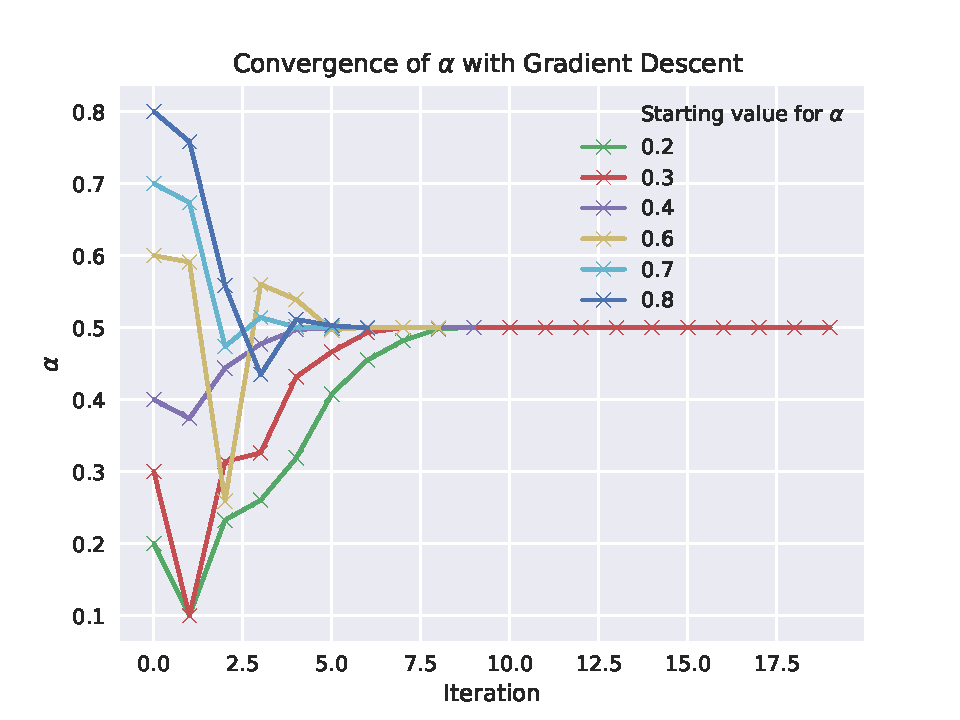
\includegraphics{figures/GD_NM_NIA.pdf}
\caption{Finding the optimal $\alpha$ with GD. This plot show the number of iterations it took to reach the minimum for the non-interactive spherical trap.}\label{fig:gd_nm_nia}
\end{figure} 

\begin{figure}
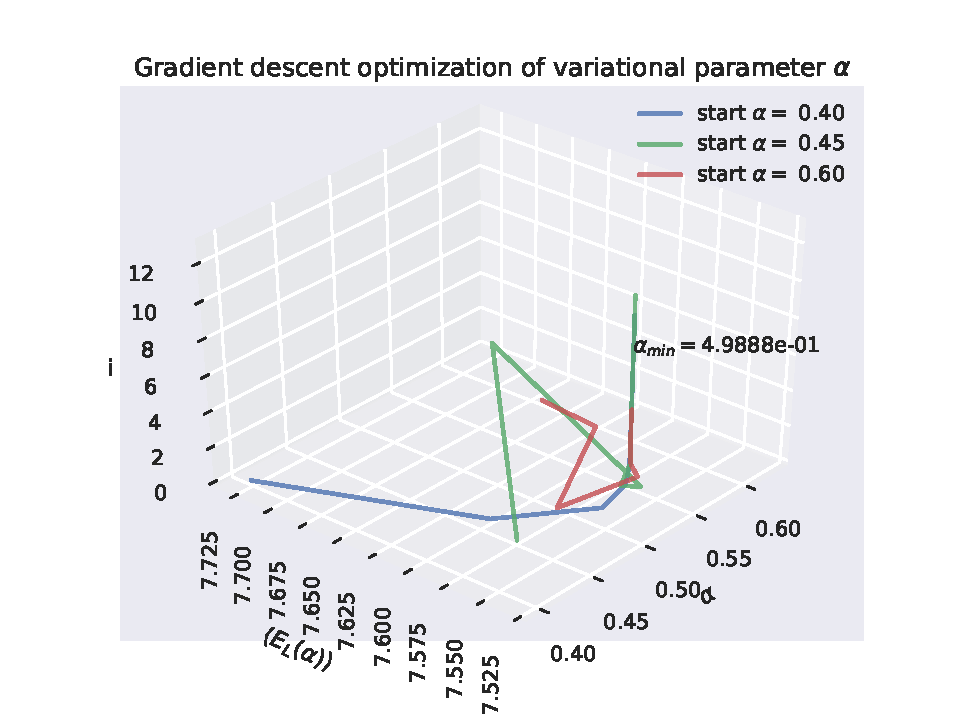
\includegraphics{figures/GD_NM_IA.pdf}
\caption{Finding the optimal $\alpha$ with GD. This plot shows the first central moment for the local energy on the y-axis, the variational parameter on the x axis and the GD iteration number on the z-axis for the interactive spherical trap. We observe that the GD algorithm finds a satisfyingly stable minimum with few iterations}\label{fig:gd_nm_ia}
\end{figure} 

\subsection*{\textbf{1g:} Onebody densities}

The onebody density was computed by counting particles in equipartitioned bins around the origo. The origo was chosen as a referemce because it is the natural focal point of particles in the harmonic oscillator trap we implemented. The bins were equipartitioned by a set step length trivially determined as $\Delta L = L/n_{bins}$ where $L$ denotes the endpoint of the interval and $n_{bins}$ the total number of bins. Each of those bins were normalized by the total count number and a factor corresponding to the difference in physical space occupied by each bin i.e. $1$ for the $1D$ case, $r$ for the $2D$ case and finally $r^2$ for the $3D$ case. The implementation of the algorithm can be found in \lstinline{vmc.cpp}. A simulation was run to compute the onebody densities for both the interactive and non-interacitve case for the respective minimas of the variational parameter $\alpha$. The result of this simulation is shown in figure \ref{fig:obd_i_ni} \footnote{at commit \lstinline{c9c91eaaaadf97f48e5130ab927667038eebcfcc}} 

\begin{figure}
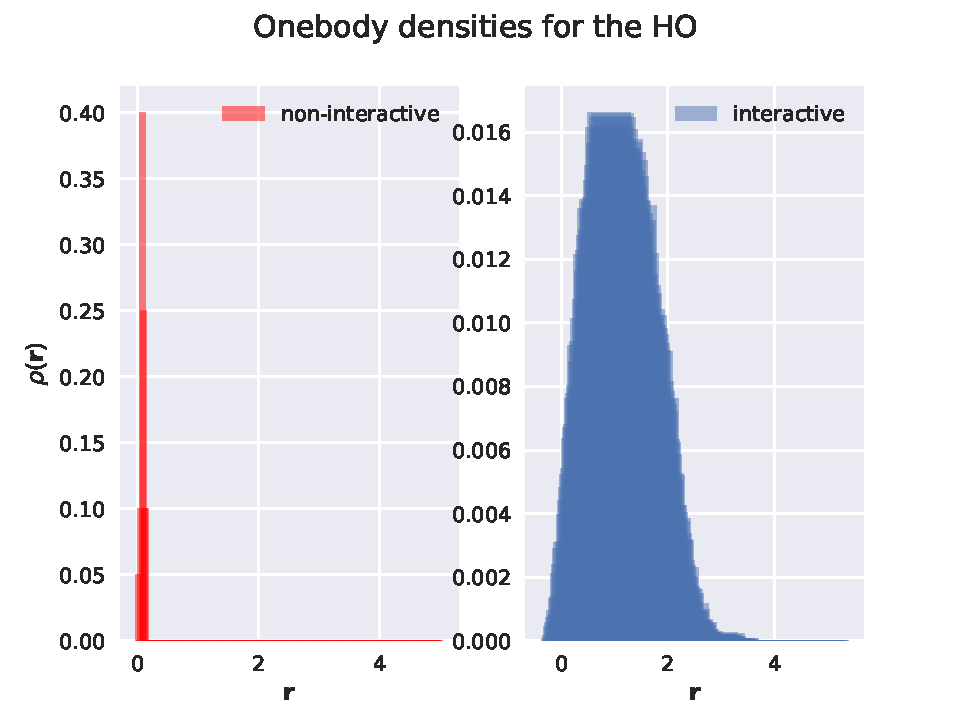
\includegraphics{figures/obd_i_ni.pdf}
\caption{With the optimal parameters for alpha the onebody densities are computed and shown above. We observe that the jastrow factor has a large and pronounced effect on the relative distribution of particles. Additionally we note that for the non-interactive case we expect a density that approximates a delta function as figuratively all bosons will be in the HO ground state.}\label{fig:obd_i_ni}
\end{figure} 
\section{Discussion}
\subsection{Brute force metropolis}

Using the simplest version of the metropolis algorithm we've shown good results for the convergence towards analytical values for two non-interactive fermions. In comparison to a more traditional VMC method we encounter more typical machine learning problems. Working with hyperparameters like $\gamma$ and the magnitude of the sampling step in the metropolis algorithm exposes (especially with importance sampling) problems with glassy energy landscapes. Wherein the optimum is fairly localized and close to zero outside leading to gradient descent breaking down. We did not explore methods to remedy this problemm, though it should be noted  that this exists in the literature.  While the tuning of the variational parameters are fairly expensive for two particles how the method scales is the  true test of it's efficacy in the field. 

\subsection{Importance sampling}


\subsection{Gibbs sampling}

\subsection{The interactive case}

We observe that the importance sampling algorithm was very sensitive to the tuning of hyperparameters and we were not able to get the gibbs-sampler to perform even for the non-interactive case we opted to use the brute force method to investicate the interactive case of two fermions. The brute force method achieves great, but spurious accuracy as it touches the analytic minimum of 3 a.u. but does not hold this solution and averages at about $3.1$ a.u. with a standard deviation of about $0.2$. This estimate does not seem wholly unreasonable  and we can conclude that using a generative method as a replacement to a more traditional ansatz of the wavefunction may not be optimal but is at least feasible. 
\section{Conclusion}
In this project we've shown the possible use cases of a generative machine learning algorithm applied to a simple many-body phyisics problem. For two non-interactive fermions we've shown convergence to analytical values when simulatig with a VMC + RBM model with a simple metropolis algorithm. Further  we implemented two different sampling schemes to try and improve the model. From our results it would seem importance sampling is very sensitive to the hyper-parameters of the model while we were unable to produce satisfactory results with the gibbs sampler at all. 
\appendix
\section{Figures}
\subsection{1f)}\label{app:fig}

\begin{figure}
\hspace{-2.8cm}
\begin{tabular}{cc}
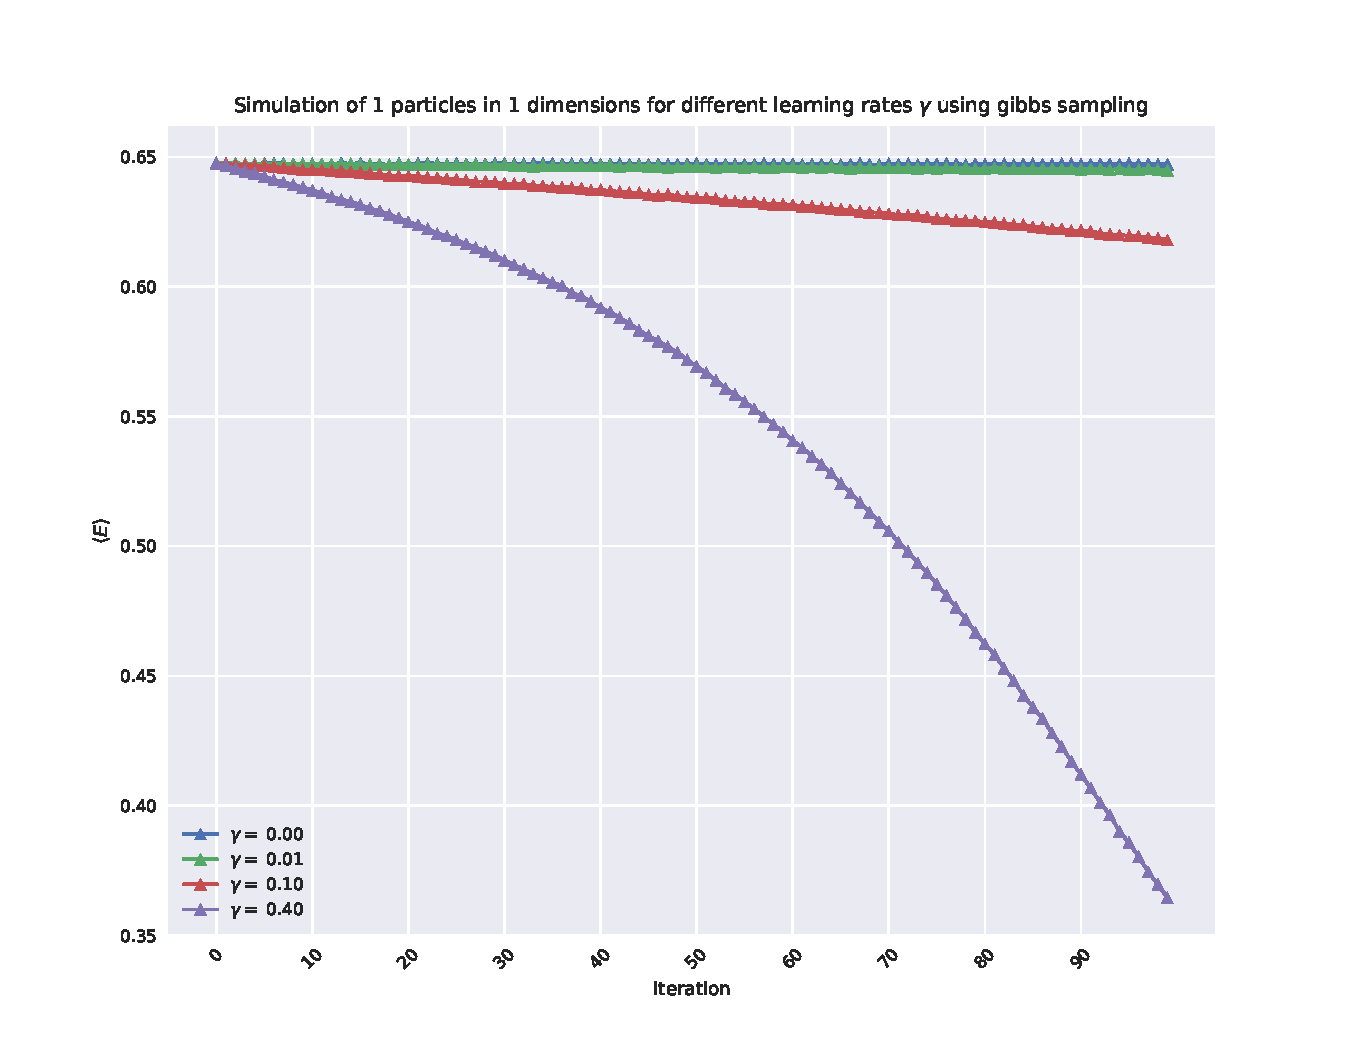
\includegraphics[width = 0.5\paperwidth]{figures/gibbs_1p_1d_N2.pdf} & 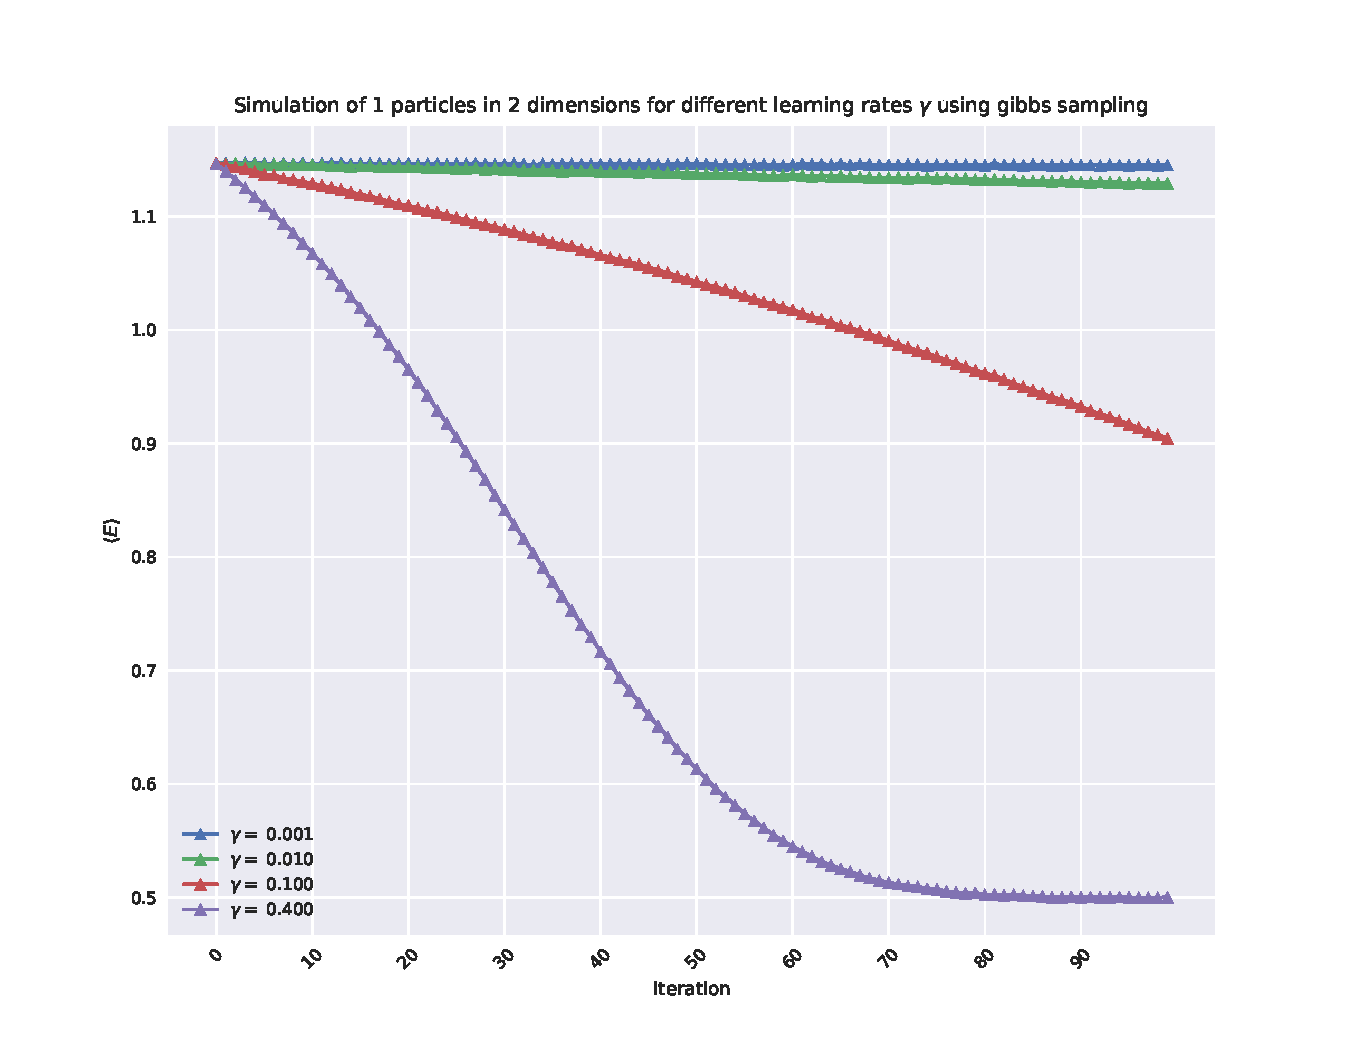
\includegraphics[width = 0.5\paperwidth]{figures/gibbs_1p_2d_N3.pdf} \\
\multicolumn{2}{c}{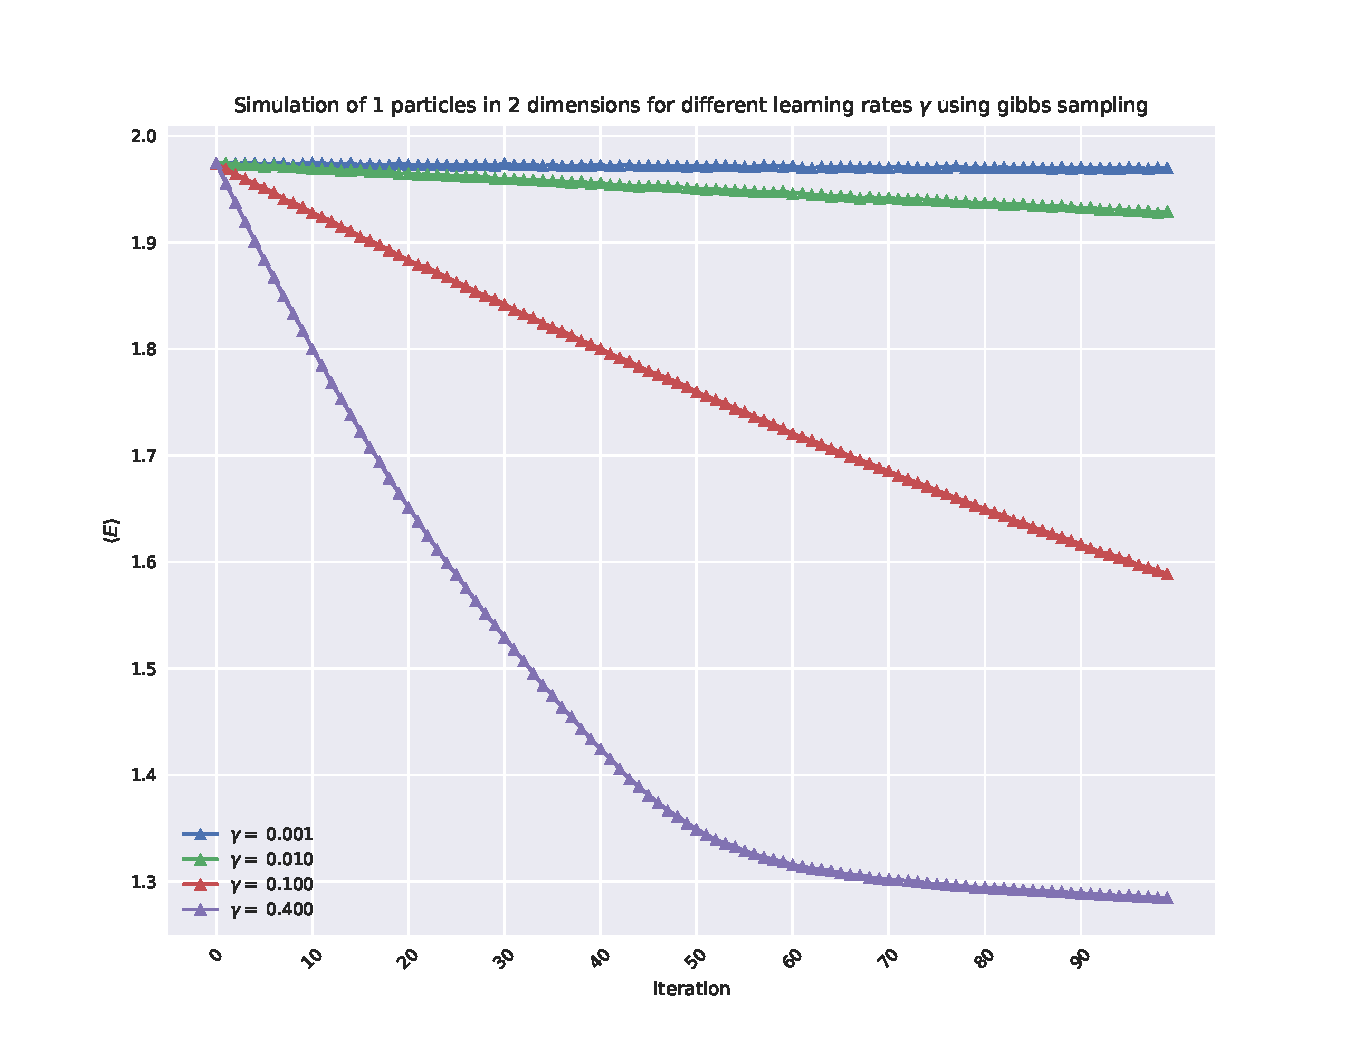
\includegraphics[width=0.5\paperwidth]{figures/gibbs_1p_3d_N4.pdf} }
\end{tabular}
\caption{Plots for simulations with 1 particle and 1-3 dimensions using Gibbs sampling with different training rate values. Number of simulations for optimizing parameters are showed in x-axis.(The lowest figure is for 1 particle in 3 dimensions, wrong title.)}
\label{fig:1f_1}
\end{figure}

\begin{figure}
\hspace{-2.8cm}
\begin{tabular}{cc}
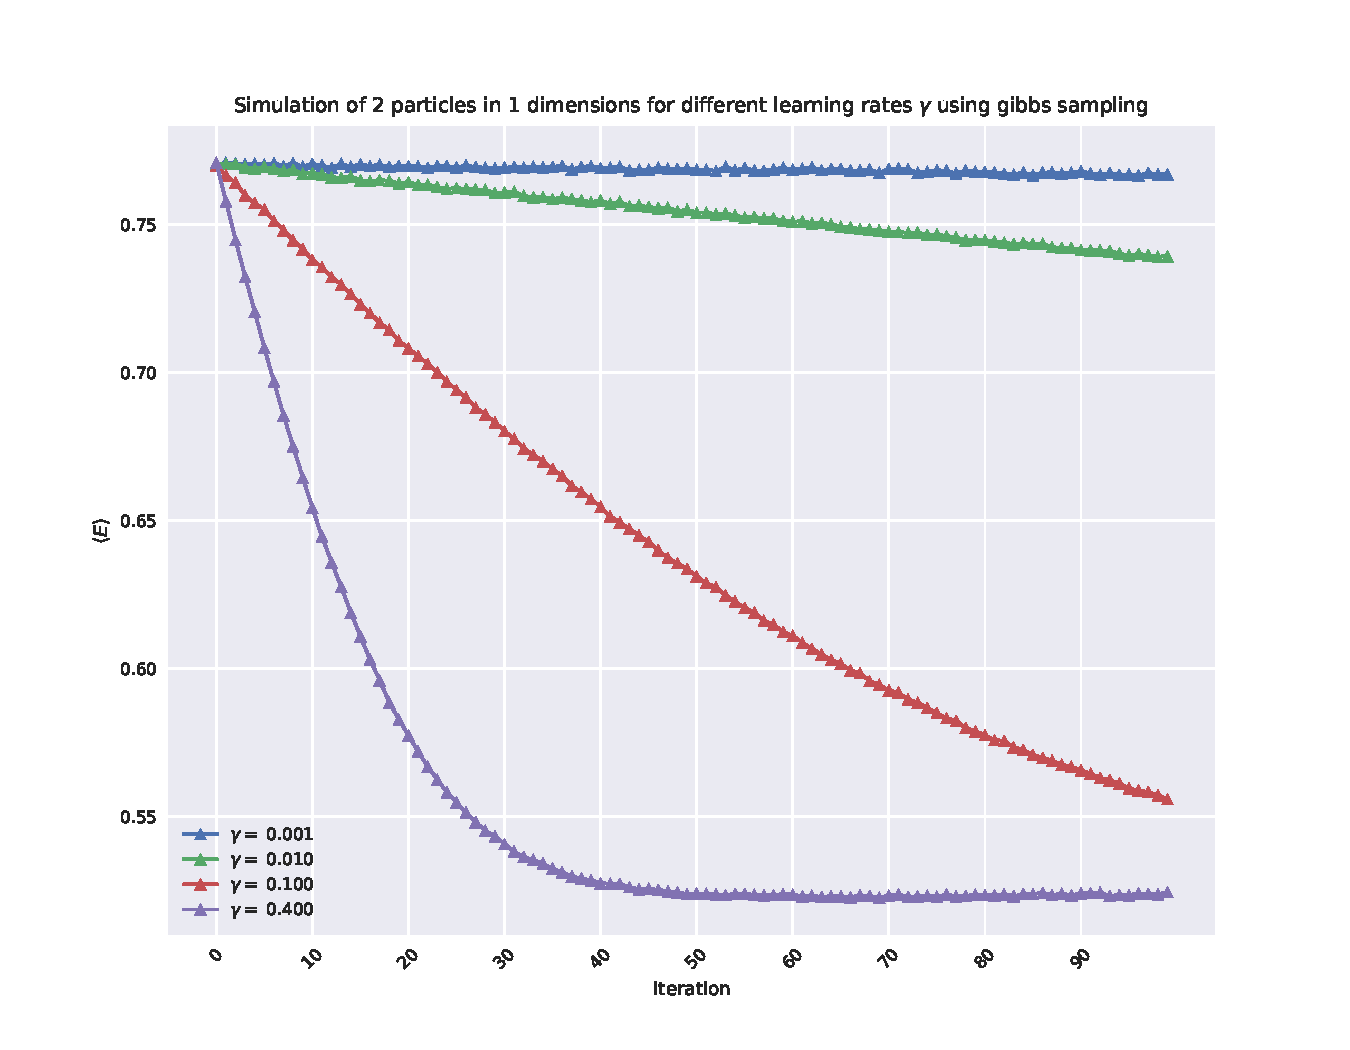
\includegraphics[width = 0.5\paperwidth]{figures/gibbs_2p_1d_N3.pdf} & 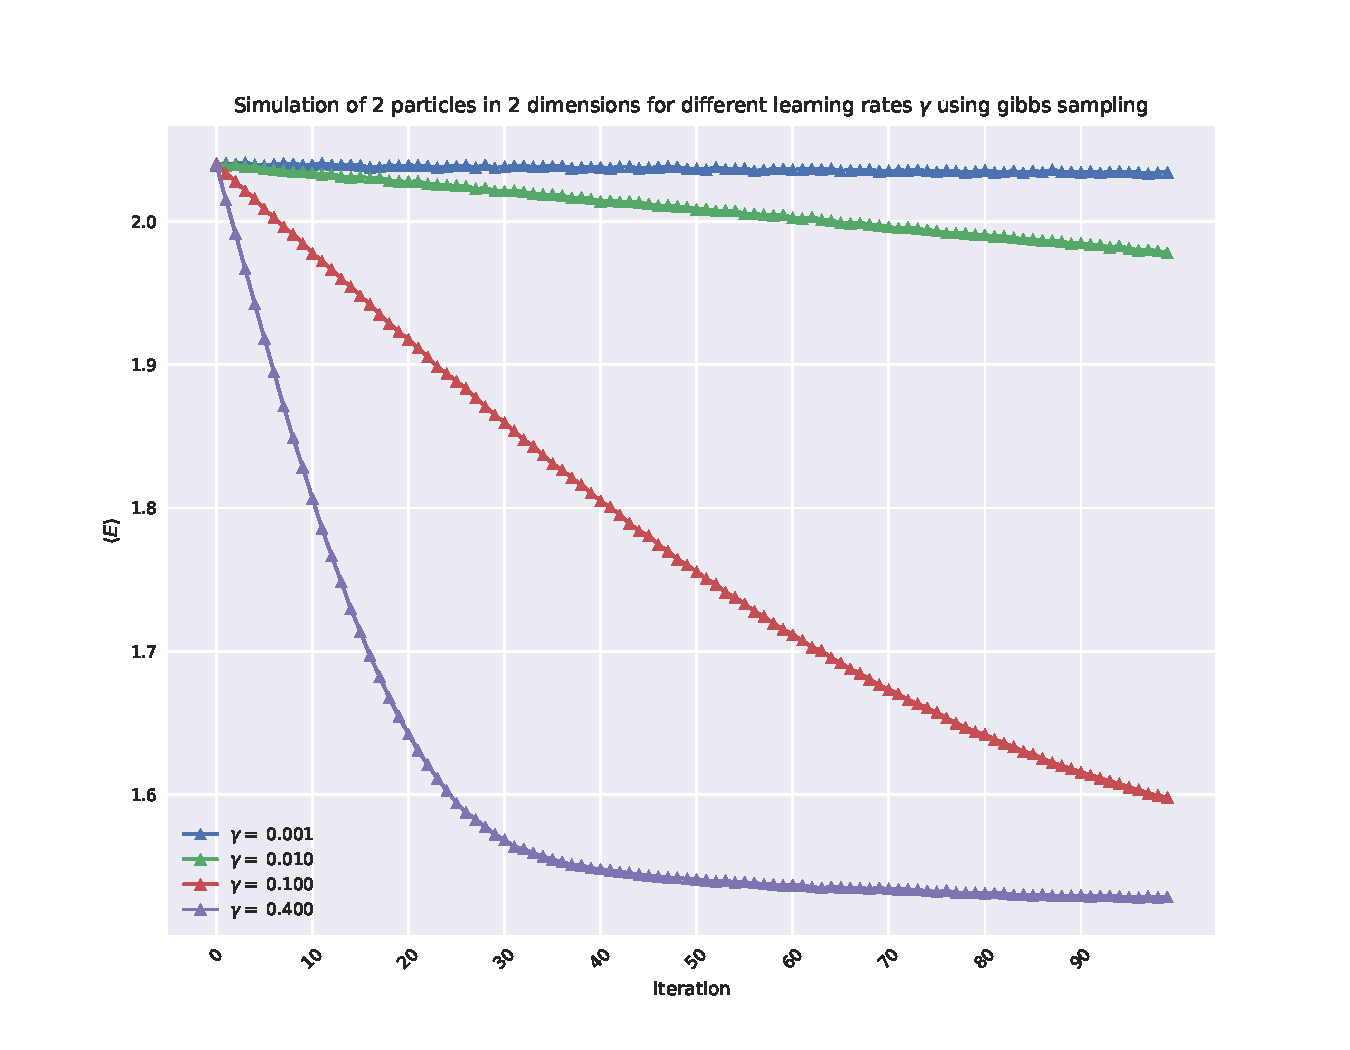
\includegraphics[width = 0.5\paperwidth]{figures/gibbs_2p_2d_N4.pdf} \\
\multicolumn{2}{c}{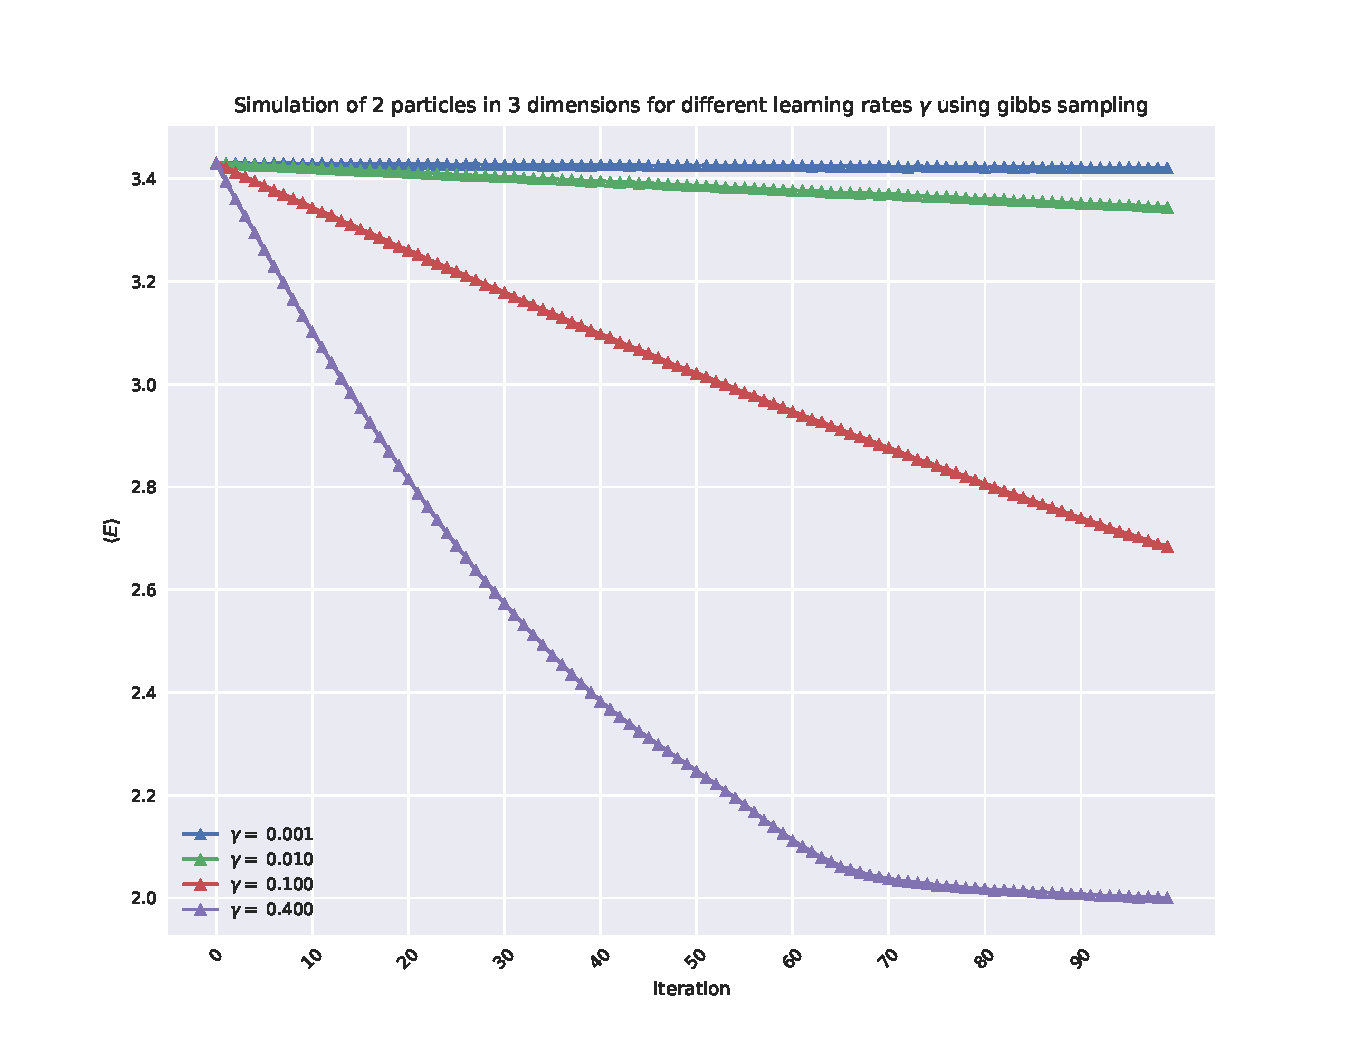
\includegraphics[width=0.5\paperwidth]{figures/gibbs_2p_3d_N8.pdf} }
\end{tabular}
\caption{Plots for simulations with 2 particle and 1-3 dimensions using Gibbs sampling with different training rate values. Number of simulations for optimizing parameters are showed in x-axis.}
\label{fig:1f_2}
\end{figure}

\begin{figure}
\hspace{-2.8cm}
\begin{tabular}{c}
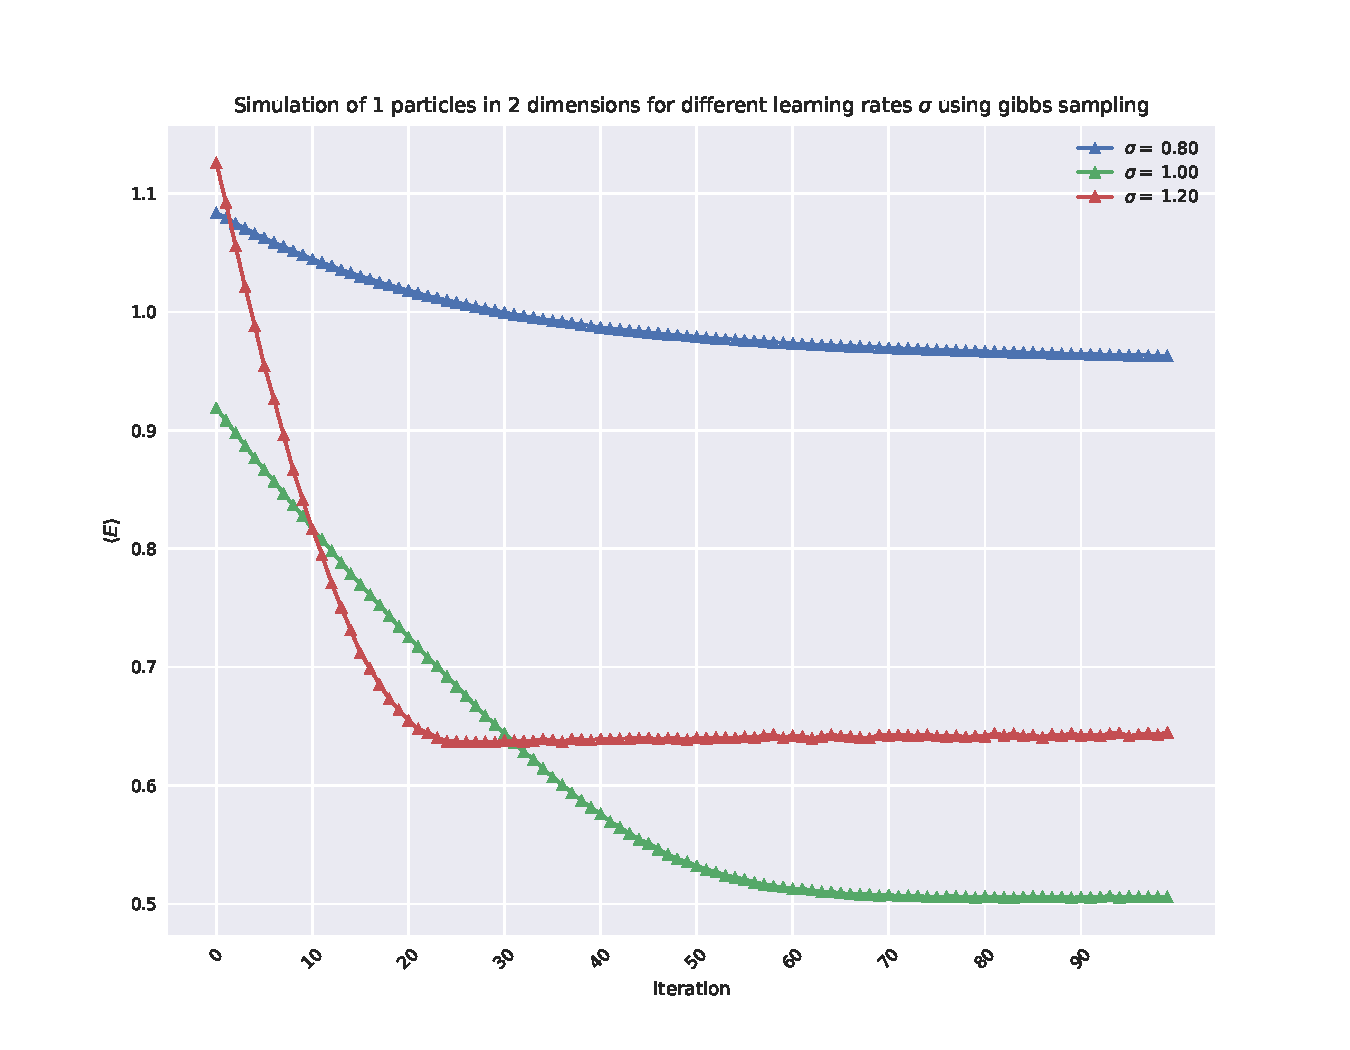
\includegraphics[width = 1.0\paperwidth]{figures/gibbs_08_1_12_gamma04.pdf}\\
\end{tabular}
\caption{Plot of simulation with 1 particle in 2 dimensions using Gibbs sampling with different standard deviation of the nois of the visible nodes, $\sigma$.}
\label{fig:1f_3}
\end{figure}

\section{Figures for brute force metropolis and importance sampling}
\begin{figure}[h]
\hspace{-2.8cm}
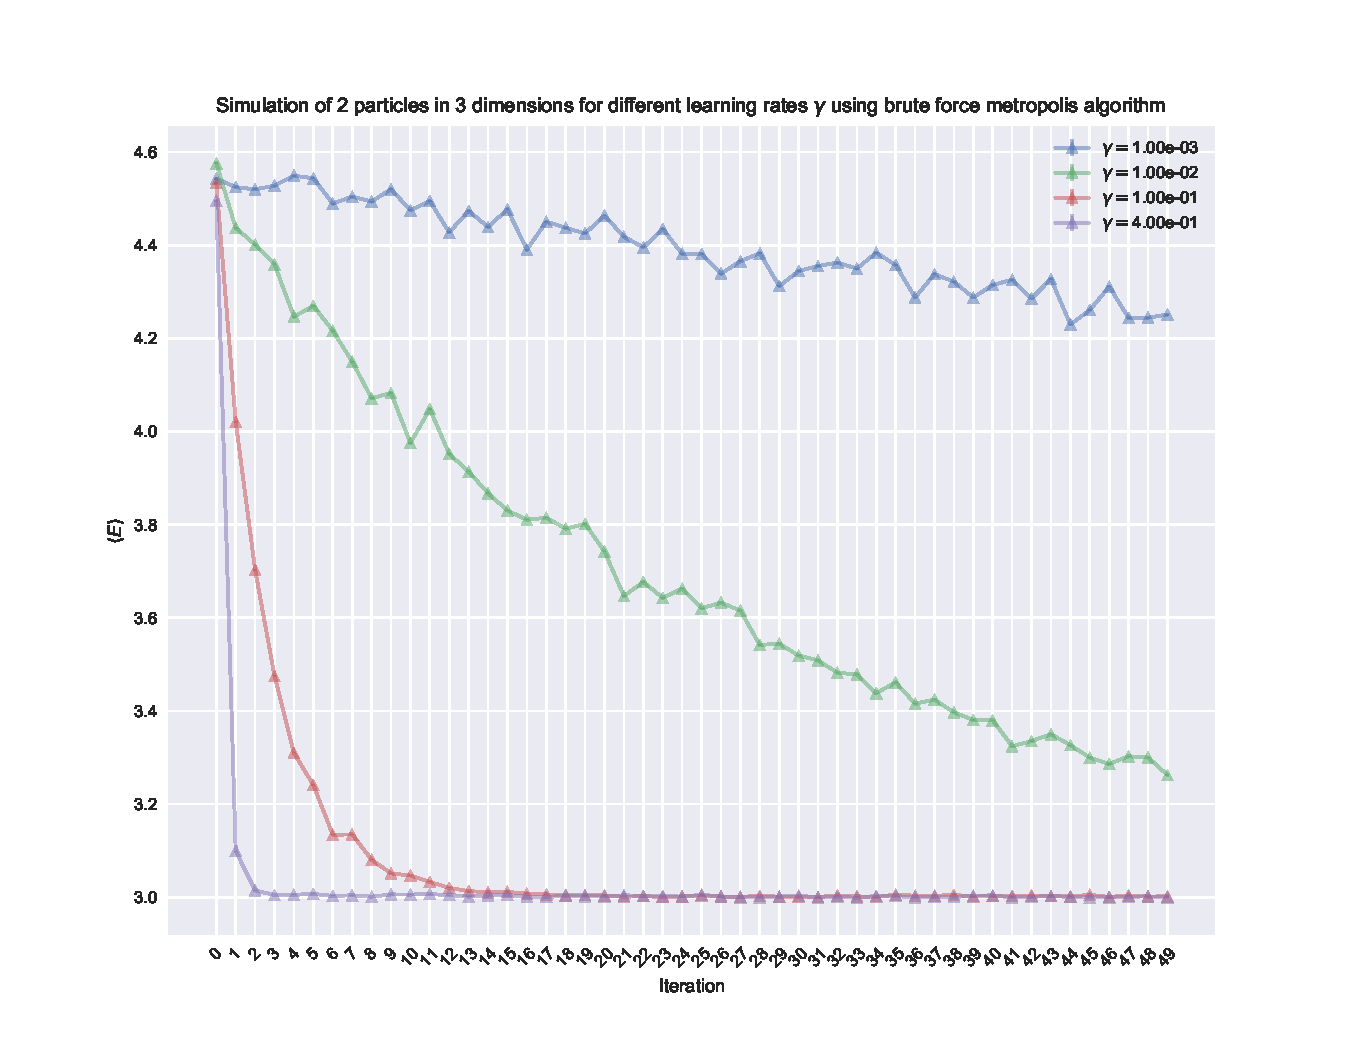
\includegraphics[width = \paperwidth]{figures/naive_2p_3d.pdf}
\caption{Plot of simulation with 2 particles in 3 dimensions with varied learning rates $\gamma$, using brute force metropolis sampling.
			2 hidden nodes were used.
			For detailed values on energy, variance, and CPU-time per mc-cycle, see table \ref{tab:naive-nin}}
\label{fig:naive-nin}
\end{figure}


\begin{figure}[h]
\hspace{-2.8cm}
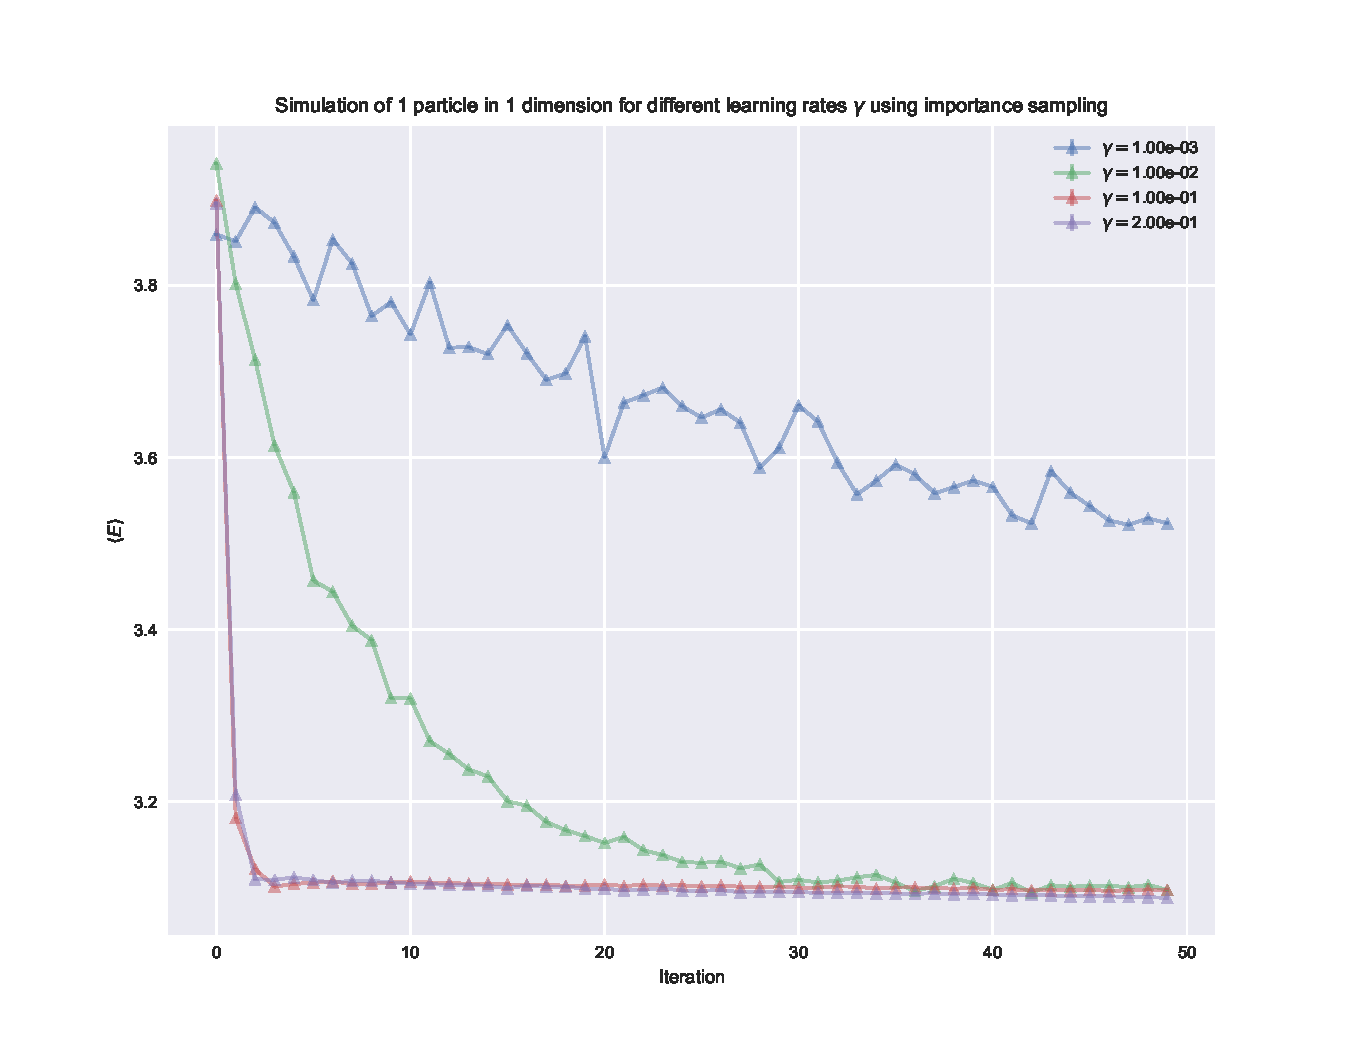
\includegraphics[width = \paperwidth]{figures/importance_2p_3d.pdf}
\caption{Plot of simulation with 2 particles in 3 dimensions with varied learning rates $\gamma$, using brute force metropolis sampling.
			For detailed values on energy, variance, and CPU-time per mc-cycle, see table \ref{tab:importance-nin-gamma}}
\label{fig:importance-nin-gamma}
\end{figure}


\begin{figure}[h]
\hspace{-2.8cm}
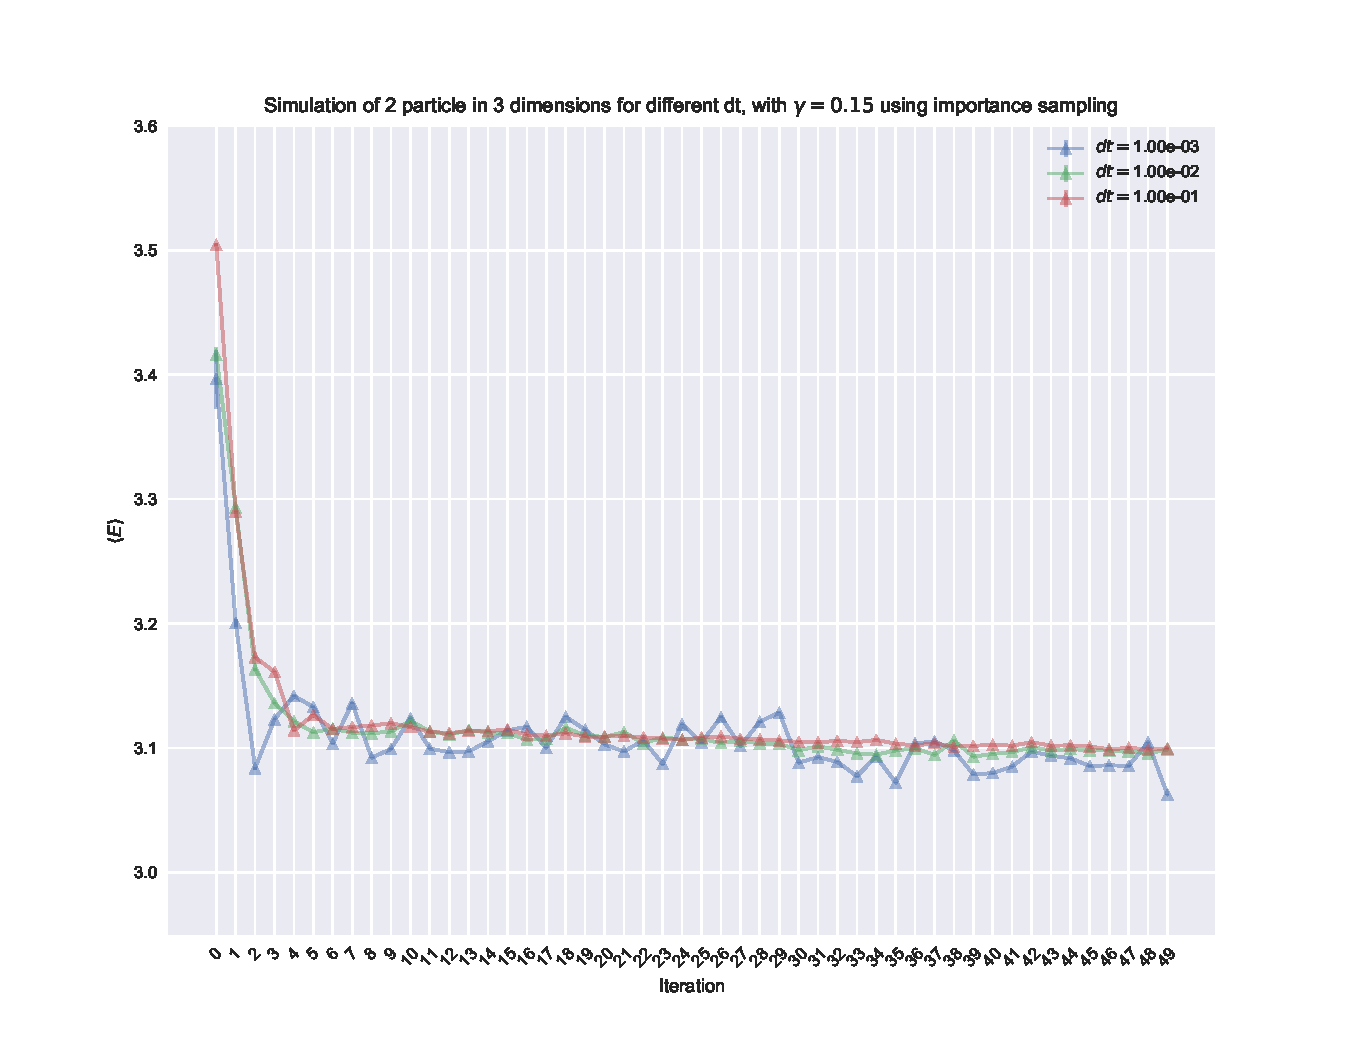
\includegraphics[width = \paperwidth]{figures/importance_2p_3d_dt.pdf}
\caption{Plot of simulation with 2 particles in 3 dimensions with varied learning rates $\gamma$, using brute force metropolis sampling.
			For detailed values on energy, variance, and CPU-time per mc-cycle, see table \ref{tab:importance-nin-dt}}
\label{fig:importance-nin-dt}
\end{figure}

\section{Local energy with $\psi(x) = F_{rbm}$}

Given the Hamiltonian in eq. \ref{eq:Hamilt} the expression for the local energy is given by the following.

\begin{align*}
E_L &= \frac{1}{\Psi}\hat{H}\psi \\
&= \sum_{k}^{P} \frac{1}{2} \left( -\frac{1}{\Psi} \nabla_k^2 \Psi +  \omega^2 r_k^2 \right) + \sum_{k < l} \frac{1}{r_{kl}}
\end{align*}

We wish to find the Laplacian of the NQS wave function. Since our visible nodes represents the particle positions in Cartesian coordinates the Laplace operator takes the second partial derivative with respect to each independent variable in the vector space. It can therefore be written as  

\begin{equation*}
\nabla_k^2 \Psi = \sum_{l}^{D} \frac{\partial^2}{\partial x_{kl}^2} \Psi.
\end{equation*}

\begin{equation*}
E_L = \sum_{k}^{P} \sum_{l}^{D} \frac{1}{2} \left( -\frac{1}{\Psi} \frac{\partial^2}{\partial x_{kl}^2} \Psi +  \omega^2 r_k^2 \right) + \sum_{k < l} \frac{1}{r_{kl}}
\end{equation*}

\begin{equation*}
E_L = \sum_{i}^{M} \frac{1}{2} \left( -\frac{1}{\Psi} \frac{\partial^2}{\partial X_{i}^2} \Psi +  \omega^2 X_i^2 \right) +  \sum_{k < l} \frac{1}{r_{kl}}
\end{equation*}

In the above equation we have used the fact that the number of visible nodes are $M = P \cdot D$. This reduces the number of sums in the first term to one. Also we see that it would be an advantage to solve the derivatives of $\ln \Psi$ since our wave function consist of sums in the exponential and also removes the $\Psi$ in the denominator. Thus the identity below is helpful. 

\begin{equation*}
\frac{1}{\Psi} \frac{\partial^2}{\partial X_{i}^2} \Psi = \left( \frac{\partial}{\partial X_{i}} \ln \Psi \right)^2 + \frac{\partial^2}{\partial X_{i}^2} \ln \Psi
\end{equation*}


\begin{equation*}
E_L = \sum_{i}^{M} \frac{1}{2} \left( - \left( \frac{\partial}{\partial X_{i}} \ln \Psi \right)^2 + \frac{\partial^2}{\partial X_{i}^2} \ln \Psi  + \omega^2 X_i^2 \right) +  \sum_{k < l} \frac{1}{r_{kl}}
\end{equation*}

Our local energy can be rewritten and we must now solve both the first and second derivative of the wave function. Our wave function is represented by the marginal probability $F_{rbm}$.

\begin{align*}
\Psi(X) &= F_{rbm}(X) \\
&= \frac{1}{Z} \exp \left( -\sum_{i}^{M} \frac{(X_i - a_i)^2}{2 \sigma^2} \right) \prod_{j}^{N} \left( 1 + \exp \left( b_j + \sum_{i}^{M} \frac{X_i \omega_{ij}}{\sigma^2} \right) \right)
\end{align*}


\begin{equation*}
\ln \Psi = -\ln Z - \sum_{i}^{M} \frac{(X_i - a_i)^2}{2 \sigma^2} +  \sum_{j}^{N} \ln \left(1 + \exp \left( b_j + \sum_{i}^{M} \frac{X_i \omega_{ij}}{\sigma^2} \right) \right)
\end{equation*}

Since $Z$ is the normalization constant its derivative is zero and can be removed.
We end up with the following

\begin{align*}
\nabla_i \ln \Psi &= \nabla_i \left( - \sum_{i}^{M} \frac{(X_i - a_i)^2}{2 \sigma^2} +  \sum_{j}^{N} \ln \left( 1 + \exp \left( b_j + \sum_{i}^{M} \frac{X_i \omega_{ij}}{\sigma^2} \right) \right) \right) \\
&= \frac{\partial}{\partial X_i} \left( - \sum_{i}^{M} \frac{(X_i - a_i)^2}{2 \sigma^2} +  \sum_{j}^{N} \ln \left(1 + \exp \left( b_j + \sum_{i}^{M} \frac{X_i \omega_{ij}}{\sigma^2} \right) \right) \right)\\
&= \frac{-2 (X_i - a_i) 2 \sigma^2}{(2 \sigma^2)^2} + \sum_{j}^{N} \frac{1}{1 + \exp \left( b_j + \sum_{i}^{M} \frac{X_i \omega_{ij}}{\sigma^2} \right)} \left( \frac{\omega_{ij}}{\sigma^2} \right) \exp \left(  b_j + \sum_{i}^{M} \frac{X_i \omega_{ij}}{\sigma^2} \right) \\
&= \frac{-(X_i - a_i)}{\sigma^2} + \frac{1}{\sigma^2}\sum_{j}^{N} \frac{\omega_{ij}}{1 + \exp \left( -b_j - \sum_{i}^{M} \frac{X_i \omega_{ij}}{\sigma^2} \right)}
\end{align*}

Given the first derivative we now find the second derivative. And we have solved the analytic case of the local energy.

\begin{align*}
\nabla_i^2 \ln \Psi &= \nabla_i^2 \left( - \sum_{i}^{M} \frac{(X_i - a_i)^2}{2 \sigma^2} +  \sum_{j}^{N} \ln \left( 1 + \exp \left( b_j + \sum_{i}^{M} \frac{X_i \omega_{ij}}{\sigma^2} \right) \right) \right) \\
&= \frac{\partial}{\partial X_i} \left( \frac{-(X_i - a_i)}{\sigma^2} + \frac{1}{\sigma^2} \sum_{j}^{N} \frac{\omega_{ij}}{1 + \exp \left( -b_j - \sum_{i}^{M} \frac{X_i \omega_{ij}}{\sigma^2} \right)} \right) \\
&= -\frac{1}{\sigma^2} + \frac{1}{\sigma^2} \sum_{j}^{N} \frac{-\omega_{ij}}{\left(1 + \exp \left( -b_j - \sum_{i}^{M} \frac{X_i \omega_{ij}}{\sigma^2} \right)\right)^2} \left( \frac{-\omega_{ij}}{\sigma^2} \right) \exp \left( -b_j - \sum_{i}^{M} \frac{X_i \omega_{ij}}{\sigma^2} \right) \\
&= -\frac{1}{\sigma^2} + \frac{1}{\sigma^4} \sum_{j}^{N} \frac{\left(\omega_{ij}\right)^2  }{\left(1 + \exp \left( -b_j - \sum_{i}^{M} \frac{X_i \omega_{ij}}{\sigma^2} \right)\right)^2}\exp \left( -b_j - \sum_{i}^{M} \frac{X_i \omega_{ij}}{\sigma^2} \right) 
\end{align*}

\section{Gradients with respect to RMB parameters, $\psi(x) = F_{rbm}$}\label{sec:GD}

To find the local energy minimum of the NQS wavefunction the  gradient of the local energy with respect to the variational parameter $\alpha  = \{\mathbf{a}, \mathbf{b}, \mathbf{W} \}$ needs to be computed. For each variational parameter $\alpha_i \in \alpha$ the gradient is defined as in equation \ref{eq:var_grad} 

\begin{equation}\label{eq:var_grad}
G_i = \frac{\partial \expect{E_L}}{\partial \alpha_i} = 2\left( \expect{E_L \frac{1}{\Psi} \frac{\partial \Psi}{\partial \alpha_i}}  - \expect{E_L} \expect{ \frac{1}{\Psi} \frac{\partial \Psi}{\partial \alpha_i}}\right)    
\end{equation}

\noindent While the NQS is defined for the Gaussian Binary RBM as (REPLACE WITH REF TO EQ )

\begin{align*}
\Psi (\mathbf{X}) = \frac{1}{Z} \exp\left(-\sum_i^M \frac{(X_i - a_i)^2}{2\sigma^2}\right) 
    \prod_j ^N \left( 1 + \exp\left(b_j  + \sum_i^M \frac{X_i w^\mathbf{T}_{ij}}{\sigma^2}\right) \right)
\end{align*}
    
\noindent We now find it useful to use the identity 
\begin{align}
    \frac{d}{dx}\ln f(x) = \frac{1}{f(x)} \frac{d}{dx}f(x)
\end{align}

\noindent Taking the logarithm of the NQS wavefunction then gives

\begin{align}
    \ln( \Psi(\mathbf{X}) )  = \ln{\frac{1}{Z}} -\sum_i^M \frac{(X_i - a_i)^2}{2\sigma^2} 
    + \sum_j^N \ln\left[  1 + \exp\left(b_j  + \sum_i^M \frac{X_i w^\mathbf{T}_{ij}}{\sigma^2}\right) \right]
\end{align}

\noindent  The final result for the gradient of the components of $\alpha_i$ is then  

\begin{align}
    \frac{\partial \ln( \Psi(\mathbf{X}) )}{\partial a_k} &= \frac{1}{\sigma ^2} (X_k - a_k)\\
    \frac{\partial \ln( \Psi(\mathbf{X}) )}{\partial b_n} &= \left(1 +  \exp\left(- b_n  - \sum_i^M \frac{X_i w^\mathbf{T}_{in}}{\sigma^2}\right)  \right)^{-1}  \\
    \frac{\partial \ln( \Psi(\mathbf{X}) )}{\partial w_{kn}}& = \frac{X_k}{\sigma^2} \left(1 +  \exp\left(- b_n  - \sum_i^M \frac{X_i w^\mathbf{T}_{in}}{\sigma^2}\right)  \right)^{-1}   
\end{align}

\section{Local energy with $\psi(x) = \sqrt{F_{rbm}}$}

In the case of the Gibbs sampling we represent the wave function as 

\begin{align*}
\Psi(X) &= \sqrt{F_{rbm}(X)} \\
&= \sqrt{\frac{1}{Z} \exp \left( -\sum_{i}^{M} \frac{(X_i - a_i)^2}{2 \sigma^2} \right) \prod_{j}^{N} \left( 1 + \exp \left( b_j + \sum_{i}^{M} \frac{X_i \omega_{ij}}{\sigma^2} \right) \right)}.\\
\end{align*}

Which is simply reduced to a constant in front of the term when taking the natural logarithm of the wave function.

\begin{equation*}
\ln \Psi = -\frac{1}{2} \left( \ln Z - \sum_{i}^{M} \frac{(X_i - a_i)^2}{2 \sigma^2} +  \sum_{j}^{N} \ln \left(1 + \exp \left( b_j + \sum_{i}^{M} \frac{X_i \omega_{ij}}{\sigma^2} \right) \right) \right)
\end{equation*}

Now we can easily see that the derivatives of the logarithm of the nqs wave function becomes,

\begin{align*}
\nabla_i \ln \Psi &= \nabla_i \left( - \sum_{i}^{M} \frac{(X_i - a_i)^2}{4 \sigma^2} +  \frac{1}{2} \sum_{j}^{N} \ln \left( 1 + \exp \left( b_j + \sum_{i}^{M} \frac{X_i \omega_{ij}}{\sigma^2} \right) \right) \right) \\
&= \frac{-(X_i - a_i)}{2\sigma^2} + \frac{1}{2\sigma^2}\sum_{j}^{N} \frac{\omega_{ij}}{1 + \exp \left( -b_j - \sum_{i}^{M} \frac{X_i \omega_{ij}}{\sigma^2} \right)},
\end{align*}


\begin{align*}
\nabla_i^2 \ln \Psi &= \nabla_i^2 \left( - \sum_{i}^{M} \frac{(X_i - a_i)^2}{4 \sigma^2} +  \frac{1}{2} \sum_{j}^{N} \ln \left( 1 + \exp \left( b_j + \sum_{i}^{M} \frac{X_i \omega_{ij}}{\sigma^2} \right) \right) \right) \\
&= -\frac{1}{2\sigma^2} + \frac{1}{2\sigma^4} \sum_{j}^{N} \frac{\left(\omega_{ij}\right)^2  }{\left(1 + \exp \left( -b_j - \sum_{i}^{M} \frac{X_i \omega_{ij}}{\sigma^2} \right)\right)^2}\exp \left( -b_j - \sum_{i}^{M} \frac{X_i \omega_{ij}}{\sigma^2} \right) 
\end{align*}

and are the derivative to be replaced in the expression of the local energy when we employ the Gibbs sampling.

\section{Gradients with respect to RMB parameters, $\psi(x) = \sqrt{F_{rbm}}$}

We also need to update the gradients to be used in the gradient descent method. These are also easily found, a simple constant i front of each term.


\begin{align}
\frac{\partial \ln( \Psi(\mathbf{X}) )}{\partial a_k} &= \frac{1}{2 \sigma ^2} (X_k - a_k)\\
\frac{\partial \ln( \Psi(\mathbf{X}) )}{\partial b_n} &= \frac{1}{2}\left(1 +  \exp\left(- b_n  - \sum_i^M \frac{X_i w_{in}}{\sigma^2}\right)  \right)^{-1}  \\
\frac{\partial \ln( \Psi(\mathbf{X}) )}{\partial w_{kn}}& = \frac{X_k}{2 \sigma^2} \left(1 +  \exp\left(- b_n  - \sum_i^M \frac{X_i w_{in}}{\sigma^2}\right)  \right)^{-1}   
\end{align}


\bibliographystyle{unsrt}
\bibliography{bibliography}

\end{document}
